%\section{Rectangles \hfill 11 pts.  \Clocklogo 50'}

On souhaite programmer un �diteur graphique qui permet de dessiner des rectangles sur un plan muni d'un rep�re cart�sien.

Un rectangle est d�fini par :
\begin{itemize}
\item un \textsf{point} sur le plan qui repr�sente son coin sup�rieur gauche ;
\item une \textsf{longueur} ;
\item une \textsf{largeur} ;
\item et une \textsf{couleur} qui peut �tre  blanche, noire ou grise.
\end{itemize} 

 Un point \textsf{P}  est d�fini par un couple de r�els :
 \begin{itemize}
 \item  \textsf{x} appel� l'abscisse de \textsf{P} ;
\item   \textsf{y} appel� l'ordonn�e de \textsf{P}.
 \end{itemize}


\begin{enumerate}
%\vspace{.25cm}
\item D�finir la structure {\textsf{Rectangle}}.  \hfill  \textbf{3 pts} 

%##########
\solution
\begin{center}
\begin{minipage}{.7\textwidth}
 %footnotesize
  \lstinputlisting[firstline=1,lastline=20]{Rectangls.c}
 \end{minipage}
 \end{center}

%\vspace{.25cm}
\item \'Ecrire une fonction {\textsf{saisir\_Rectangle}}. \hfill \textbf{2 pts} 

%##########
\solution
\begin{center}
\begin{minipage}{.7\textwidth}
 %footnotesize
  \lstinputlisting[firstline=25,lastline=40]{Rectangls.c}
 \end{minipage}
 \end{center}
 
%\vspace{.25cm}
\item  \'Ecrire une fonction {\textsf{deplacer}} qui prend en entr�e un rectangle R et un point P$\prime$ et puis elle d�place le rectangle R vers le point P$\prime$. Par exemple, le rectangle R1 prendra la place du rectangle R2 s'il est  d�plac�  au point P'.   \hfill \textbf{1 pt} 

%##########
\solution
\begin{center}
\begin{minipage}{.7\textwidth}
 %footnotesize
  \lstinputlisting[firstline=50,lastline=53]{Rectangls.c}
 \end{minipage}
 \end{center}

%\vspace{.25cm}
\item  \'Ecrire une fonction {\textsf{zoomer}} qui prend en entr�e un rectangle et un coefficient de zoom. La fonction maintient le coin sup�rieur gauche du rectangle  puis elle agrandie ou elle rapetisse les dimensions du rectangle en fonction du coefficient du zoom.    Par exemple, le rectangle R3 devient �gale au rectangle R4 s'il est zoom�  avec un coefficient �gale � 2 et inversement R4 devient �gale � R3 s'est zoom�  avec un coefficient �gale � 0.5. \hfill \textbf{1 pt} 

%##########
\solution
\begin{center}
\begin{minipage}{.7\textwidth}
 %footnotesize
  \lstinputlisting[firstline=55,lastline=59]{Rectangls.c}
 \end{minipage}
 \end{center}

%\vspace{.25cm}
\item  \'Ecrire une fonction {\textsf{sym�trique}} qui prend en entr�e
 un rectangle R et  retourne le rectangle sym�trique 	 R$\prime$  du R par par rapport son coin sup�rieur gauche. Par exemple, le rectangle R5 est le r�sultat de l'appel de cette fonction avec le rectangle R4 comme param�tre. \hfill  \textbf{1 pt}   

%\vspace{.25cm}
%\item  \'Ecrire une fonction {\textsf{centre}} qui prend en entr�e un rectangle R et retourne le point qui se trouve � son plein milieu.  \textbf{1 pt} 

\item  \'Ecrire une fonction {\textsf{inclut}} qui prend en entr�e deux  rectangles R1 et R2   et renvoie 1 si R2 est inclus dans R1, 0 sinon. Par exemple R6 est inclus dans R7 mais R8 ne l'est pas. \hfill \textbf{2 pts} 
%##########
\solution
\begin{center}
\begin{minipage}{.7\textwidth}
 %footnotesize
  \lstinputlisting[firstline=85,lastline=93]{Rectangls.c}
 \end{minipage}
 \end{center}

%\vspace{.25cm}
\item  \'Ecrire une fonction {\textsf{inclut}} qui prend en entr�e deux  rectangles R1 et R2   et renvoie 1 si R2 est inclus dans R1, 0 sinon. Par exemple R6 est inclus dans R7 mais R8 ne l'est pas. \hfill \textbf{2 pts} 
%##########
\solution
\begin{center}
\begin{minipage}{.75\textwidth}
 %footnotesize
  \lstinputlisting[firstline=95,lastline=104]{Rectangls.c}
 \end{minipage}
 \end{center}

\begin{center}
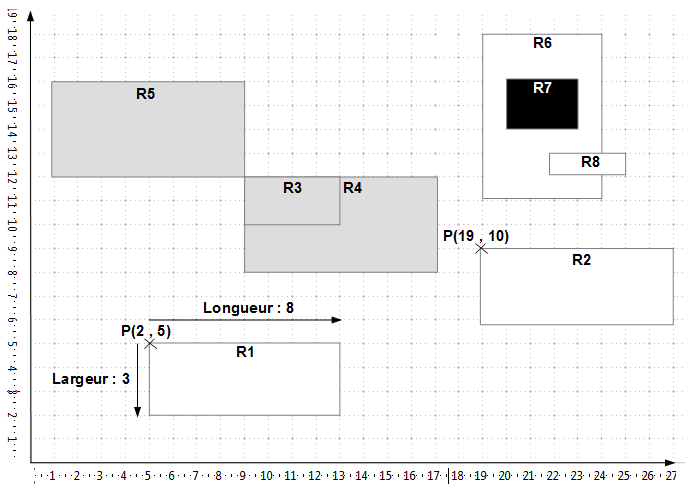
\includegraphics[width = .95\textwidth]{Rectangls.png} 
\end{center}
%\vspace{.25cm}

\item \'Ecrire une fonction \textbf{\textsf{main}} qui permet de : \hfill\textbf{1pt}
\begin{itemize}
\item d�clarer un \textsf{Graph} qui contient un ensemble de rectangles.  
\item saisir le rectangle R1 de la figure ci-dessus dans le premier rectangle de la variable \textsf{Graph}, 
\item d�placer le premier rectangle au point P$\prime(19,9)$, 
\item et enfin,  ajouter  un deuxi�me  rectangle (dans \textsf{Graph}) sym�trique au premier rectangle	 d�plac�.
\end{itemize}  
%##########
\solution
\begin{center}
\begin{minipage}{.7\textwidth}
 %footnotesize
  \lstinputlisting[firstline=150,lastline=155]{Rectangls.c}
 \end{minipage}
 \end{center}

\end{enumerate}

\endinput

\solution
\begin{center}
\begin{minipage}{.7\textwidth}
 %footnotesize
  \lstinputlisting{Rectangls.c}
%[firstline=1,lastline=10]
 \end{minipage}
 \end{center}